\documentclass[10pt]{article}

\usepackage{multirow}
\usepackage{rotating,graphicx}
%\usepackage{wrapfig}
\usepackage{amssymb}
\usepackage{amsmath}
\usepackage{lscape}
\usepackage{times}
\usepackage{color}  % For \textcolor and \color % Ex. : \textcolor{red}{Text colored with} ; {\color{red}Text colored with}
\usepackage{soul}   % For \hl{ highlighted text} ; \sethlcolor{colorname}
%\usepackage[table]{xcolor}
\usepackage{xcolor,colortbl}
\usepackage{capt-of}
\usepackage{textcomp}  % allows \textonehalf,  \textonequarter, or else
%\usepackage{mathcomp}  % make it math compatible

\oddsidemargin =-0.6in
\evensidemargin=-0.6in
%\textwidth=7.6in   % owl
 \textwidth=7.8in % laptop
\textheight=10.2in
% \topmargin=-.25in   % owl
 \topmargin=-1.in    % laptop
\footskip=-.0in

\newcommand{\Bl}{\ensuremath{B_{{low}}}}
\newcommand{\Bh}{\ensuremath{B_{{high}}}}
\newcommand{\Il}{\ensuremath{I_{{low}}}}
\newcommand{\Ih}{\ensuremath{I_{{high}}}}
\newcommand{\Br}{\ensuremath{B\! \rho}}
\newcommand{\CE}{concentration ellipse}
\newcommand{\CES}{CE-$\rm \mathcal{S}$}
\newcommand{\dEE}{\small \ensuremath{\frac{dE}{E}}}
\newcommand{\eg}{\ensuremath{\it e.g.}}
\newcommand{\Ha}{\ensuremath{\mathcal{H}}}
\newcommand{\Sa}{\ensuremath{\mathcal{S}}}
\newcommand{\vs}{\ensuremath{\it vs.}}
\newcommand{\ie}{\ensuremath{\it i.e.}}
\newcommand{\hbrk}{\hfill \break}
\newcommand{\sr}{synchrotron radiation}
\newcommand{\SRl}{SR loss}
\newcommand{\x}{\ensuremath{x}} 
\newcommand{\xp}{\ensuremath{{x'}}}
\newcommand{\z}{\ensuremath{z} }
\newcommand{\zp}{\ensuremath{{z'}}}
\newcommand{\y}{\ensuremath{y} }
\newcommand{\yp}{\ensuremath{{y'}}}
\newcommand{\dl}{\ensuremath{{\delta l}}} 
\newcommand{\dE}{\ensuremath{{\delta E}}}
\newcommand{\X}{\ensuremath{X} }
\newcommand{\Xp}{\ensuremath{{X'}}}
\newcommand{\Z}{\ensuremath{Z} }
\newcommand{\zg}{Zgoubi}
\newcommand{\Zp}{\ensuremath{{Z'}}}
\newcommand{\Y}{\ensuremath{Y} }
\newcommand{\Yp}{\ensuremath{{Y'}}}
\newcommand{\Len}{\ensuremath{l} }
\newcommand{\Mom}{\ensuremath{E}}
\newcommand{\Sx}{\ensuremath{\mathcal{S}_x}}
\newcommand{\Sy}{\ensuremath{\mathcal{S}_y}}
\newcommand{\Sz}{\ensuremath{\mathcal{S}_z}}

\newcommand{\C}{\ensuremath{\mathcal{C}}}
\newcommand{\D}{\ensuremath{\mathcal{D}}}
\newcommand{\HH}{\ensuremath{\mathcal{H}}}
\newcommand{\bHH}{\bar \HH}
\newcommand{\com}{{center of mass}}
\newcommand{\lab}{{laboratory frame}}
\newcommand{\LL}{\ensuremath{\mathcal{L}}}
\newcommand{\rms}{\ensuremath{rms}}
\newcommand{\wrt}{{with respect to}}

\newcommand{\bull}{\ensuremath{\bullet~}}
\newcommand{\cf}{\ensuremath{\textsl{cf.}}}
\newcommand{\bhel}{\ensuremath{\mathbf{^3He^{2+}}}}
\newcommand{\hel}{\ensuremath{\mathrm{^3He^{2+}}}}
\newcommand{\nib}{\noindent \ensuremath{\bullet~}}
\newcommand{\snib}{\noindent {\small \ensuremath{\bullet~}}}
\newcommand{\nid}{\noindent \ensuremath{\diamond~}}
\newcommand{\snid}{\noindent {\small \ensuremath{\diamond~}}}
\newcommand{\nin}{\noindent~}
\newcommand{\no}{\ensuremath{\mathbf{\vec n_0}}}
\newcommand{\MC}{Monte~Carlo}
\newcommand{\p}{\ensuremath{\mathbf{p}}}
\newcommand{\pp}{$\rm p\! \! \uparrow$}

\definecolor{orange}{rgb}{1,0.5,0}
\definecolor{yelloworange}{rgb}{1,.647,0}
\newcommand{\black}{\color{black}}
\newcommand{\red}{\color{red}}
\newcommand{\green}{\color{green}}
\newcommand{\blue}{\color{blue}}
\newcommand{\yo}{\color{yelloworange}}

\newcommand{\referenceA}{\rm  }
\newcommand{\referenceB}{\rm }
\newcommand{\referenceC}{\rm }

\pagestyle{headings}
\markboth{\small  \referenceA ~ ~   \referenceB ~ ~  \referenceC \hfill }
         {\small  \referenceA ~ ~   \referenceB ~ ~  \referenceC \hfill }


\begin{document}

\thispagestyle{empty}

\begin{minipage}{1.\linewidth}
\bf
  \flushright{F. M\'eot}
\vspace{-2ex}
  
  \flushright{BNL C-AD}
\vspace{-2ex}
  
  \flushright{Zgoubi 2019 Workshop, Boulder, CO}
\vspace{-2ex}
  
\flushright{24-29 Aug. 2019} 
\end{minipage}


\vspace{5ex}

\centerline{\LARGE \bf
 A Second Order Quadrupole Doublet Achromat
}


\section*{Recommended readings}

\nin - Sections 3.3 and 3.4 in 
``Generalization of the Zgoubi method for ray-tracing to include electric fields'',  NIM~A~340 (1994) 594-604. 

\smallskip
\nin - Zgoubi Users' Guide, regarding the keywords mentioned below (EBMULT, OBJET/KOPT=6,6[.1], etc.). Hint: use the index (last 3 pages of the Guide) to locate the related sections in Part~A and Part~B.


\smallskip
\nin - During the exercise, it is recommended to keep 2 copies of the guide at hand, with one copy opened at the Index (last 3 pages of the document).


\section*{Keywords we play with in this exercise}

EBMULT is the optical element of concern  (pp.~129 and 224 in the Users' Guide).  $ \vec B$ and $ \vec E$ are set so to ensure
focal distance as desired, and cancellation of the second order chromatic aberrations inherent to magnetic quadrupoles.

\smallskip
\noindent OBJET/KOBJ=5, 6[.1] and MATRIX will allow computing the first, second and third order transport matrices,
and series of higher order transport coefficients. 

\smallskip
\noindent REBELOTE is used to track 100,000s of particles, for statistics purposes, and FAISTORE to log them to zgoubi.fai.


\smallskip
\noindent Imaging: IMAGE is used to locate the beam waist, HISTO is used to get transverse beam densities (zpop allows
the latter as well, it can be used instead - or concurrently). 



\section*{Simulation files}

They may all be found in zgoubiFiles folder. Depending on the questions, we'll use one or the other of 
 bqpole\_image.res,  bqpole\_matrix.res,  microProbe\_matrix\_2rdOrder.res,   microProbe\_matrix\_3rdOrder.res.




\section*{Working hypotheses}

\nib The arrangement of a pair of ``E$\times$B'' quadrupoles, to form the front end of a microprobe, is sketched in the figure below. The probe is assumed to be a 20\,keV proton beam. 

\begin{minipage}{1.\linewidth}
  \centering
\begin{minipage}{0.55\linewidth}
\hspace{-0.\linewidth}
  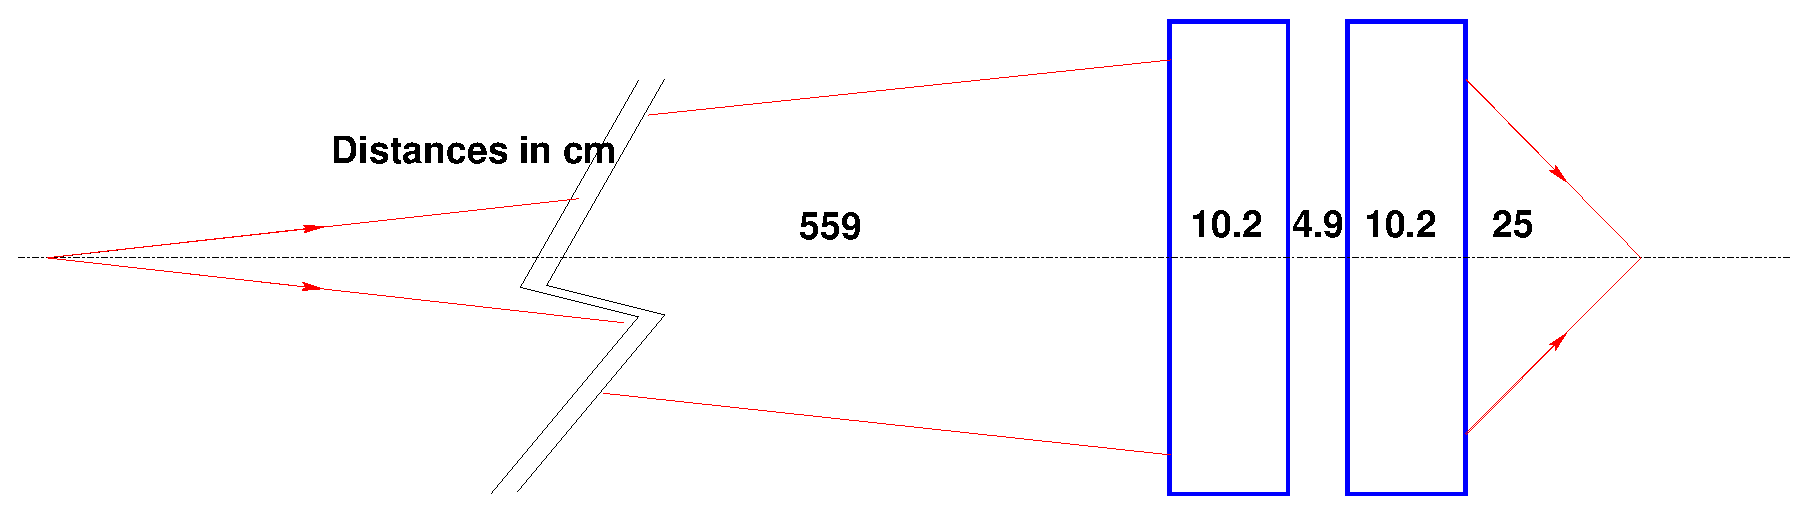
\includegraphics[width=1.\linewidth]{achromat.eps}
\end{minipage} 

\vspace{4ex}

\nin
\begin{minipage}{0.45\linewidth}
  
  {\small $\bullet$} A cross-section of the  E$\times$B quadrupole:

    \centering

  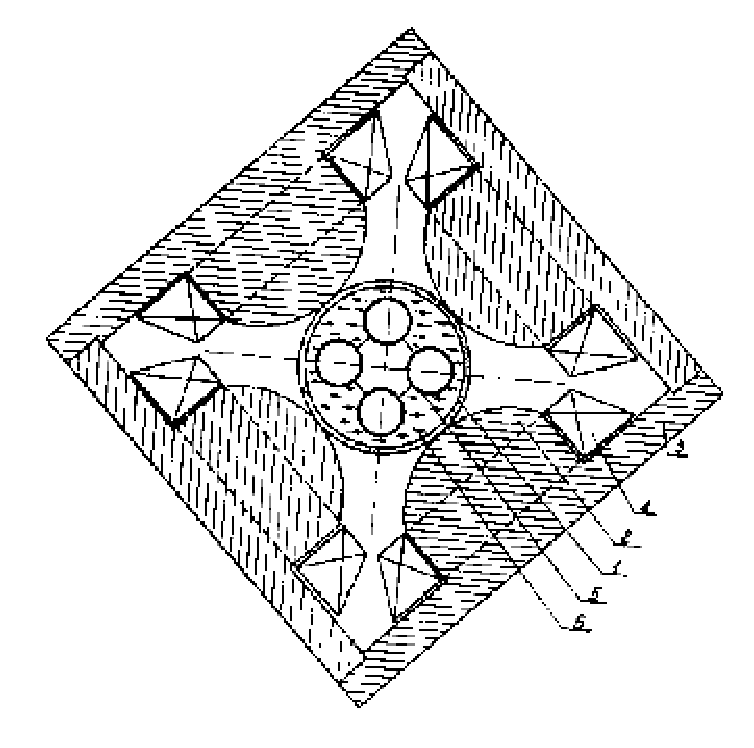
\includegraphics[width=0.28\linewidth]{EBQuad.eps}
  
                [Ref.: S.Ya.~Yavor, NIM A 26 (1964)]

  The electrostatic component (the cylindrical rods, at $\pi/4$ from the magnetic poles) satisfies: 
  
$\left\{ \begin{array}{l} E_Y = -KY = -\partial V_{el} /\partial Y \\ E_Z = +KZ = -\partial V_{el} /\partial Z \end{array} \right. $ 

                
\end{minipage} \hfill
\begin{minipage}{0.54\linewidth}
\centering
 so deriving, in the upright (Y,\,Z) frame, from the scalar potential   $V_{el} = \dfrac{K}{2}(Y^2-Z^2) \ \ \ \ (+Const)$

\medskip

In  the 45$^o$-rotated (U,\, V) frame, defined by \\[1ex]
$\left[ \begin{array}{c} U \\ V \end{array}\right]  = \left[ \begin{array}{cc} \cos 45^o & -\sin45^o \\ \sin45^o & \cos45^o\end{array} \right] \left[ \begin{array}{c} Z \\ Z \end{array}\right]$,  

~

 the equipotentials satisfy $V_{el} = K UV$.

\medskip

 
 It means that the field from an electrostatic quadrpole can be computed using the same equations as for an uprigt magnetic multipole
 (found in multip.f in zgoubi), after what the vector field so obtained must be 45$^0$-rotated (a call to XROTB at the end of
 multip.f). 
 
%Thus, the 45$^o$-rotated equipotentials of an electrostatic quad realize the same focusing effect as the equipotentials of an upright magnetic quadrupole.

\end{minipage}
\end{minipage}






\clearpage

\section*{ Numerical experience }

NOTE: Numerical parameters in the zgoubi sequence are as per sections 3.3 and 3.4 in NIM~A~340 (1994) 594-604.

~


\nin 1/ First, let's  walk through the Fortran, see what happens when the execution pointer meets 'EBMULT' in zgoubi.dat sequence...

\begin{itemize}
\item Open zgoubi\_main.f : it calls zgoubi. The rest of the it essentially manages the 'FIT' procedure.
\item Open zgoubi.f 
\begin{itemize}
  \item find include/LSTKEY.H: take a look into it, spot EBMULT -~and all of zgoubi keywords! If you need to add a keyword, that's here
  \item find 'CALL REBMUL', look into rebmul.f. What does it do?
  \item it is followed by'CALL QUASEX'. 
    Optical elements call either QUASEX, or AIMANT (check that statement, scrolling through zgoubi.f), what's the difference between the two? 
  \item  Open quasex.f.  In there, find 'CALL CHXC'. What does it do? 
  \begin{itemize}
    \item open chxc.f
    \begin{itemize}
      \item No ``EBMULT'' therein! (by contrast for instance with 'MULTIPOL', 'SOLENOID'.  Figure out why
    \end{itemize}
    \item find 'CALL TRANSF' in quasex, open transf.f: it pushes the particles, one by one, through 'INTEGR'
    \begin{itemize}
      \item find 'CALL INTEGR', open integr.f: it pushes a particle, step by step, 
        through EBMULT (or any other element)
      \item In integer.f look for 
        (i) 'CALL CHAMC',
          (ii) 'CALL CHAMK', 
          (iii) 'CALL DEVTRA': 
          Figure out what each does.
    \end{itemize}
  \end{itemize}
\end{itemize}
\end{itemize}

~

\nin 2/ Install in Zgoubi the optical sequence sketched above, leaving first the electrostatic component zero, with B value set 
to provide the image distance indicated in the figure.

Produce the transport matrices of this system, to 3rd order. 

~

\nin 3/ Now switch on the E component, setting  E and B to (i)~preserve the image distance and (ii)~ensure cancellation of second order chromatic aberrations.

Produce the transport matrices to 3rd order, compare with the previous case.

~

\nin 4/ Array sizes limited the number of particles tracked in one go ()would be increased (in the include files), 


Track 30,000 particles through the achromat in both cases above, E alone or E$\times$B.
Proceed in the following way:

- using MCOBJET, create a point object with  0.2\,mrad \textsl{rms} divergence, Gaussian, in both planes (thus, in the absence of any optical aberrations, the image would be a point). 
Add $10^{-3}$ \textsl{rms} momentum spread, Gaussian, 

- use HISTO to  display D (relative rigidity) density, as well as the initial $Y_0$ and $Z_0$ transverse beam densities, 

- use REBELOTE to iterate to $3\times 10^4$ particles,  as the maximum number of particles acceptable in MCOBJET is less (a matter of array sizing in the source code, this can be changed in [pathTo]/zgoubi-code/include/MAXTRA.H) -~by the way, how much is it?)

- use IMAGE to localize the image waist downstream of the doublet; set the final straight length to the waist distance,

- use HISTO to display the Y and Z transverse beam densities at the image.

~

\nin 5/ Repeat 4/ with B alone (as in 2/, E=0). Compare the image widths from HISTO for both cases: pure B and combined E, B.


\end{document}
